\documentclass{beamer}
\usepackage{etex}
\usetheme{Antibes}
\usepackage{amssymb,amsmath,amsthm}
\usepackage{graphicx}
\usepackage{caption}
\usepackage{subfig}
\newcommand{\bn}{\begin{enumerate}[i)]}
\newcommand{\en}{\end{enumerate}}
\newcommand{\im}{\item}
\newcommand{\CPT}[1]{\large{\textbf{CHAPTER #1}}}
\newcommand{\ir}[1]{\textbf{Remark #1}}
\newcommand{\ith}[1]{\textbf{Theorem #1}}
\newcommand{\idf}[1]{\textbf{Definition #1}}
\newcommand{\iex}[1]{\textbf{Example #1}}

%\definecolor{cardinal}{rgb}{0.77, 0.12, 0.23}
%\usecolortheme[named=cardinal]{structure}
%\setbeamercolor{block title}{bg=cardinal,fg=black}
 \usepackage{tikz}
 \usetikzlibrary{patterns,snakes,plotmarks}
 \usepackage{multirow}
% \usetikzlibrary{shadows}
\usepackage{epstopdf}
\usepackage{nicefrac}
\usepackage{lmodern}
\usepackage{pgfplots}
\usepackage{qtree}
\newcommand*{\Scale}[2][4]{\scalebox{#1}{\ensuremath{#2}}}%
\DeclareCaptionLabelSeparator{horse}{:\,\,} % change according to your needs
\captionsetup{
  labelsep = horse,
  figureposition = bottom % used to get the correct vertical space between the figure and the caption
}
\setbeamertemplate{caption}[numbered]
\setbeamertemplate{items}[circle]
\setbeamertemplate{enumerate items}[square]
\theoremstyle{definition}
\newtheorem*{exs}{Examples}
\newtheorem{ex}{Example}
\newtheorem*{exc}{Exercise}
%\usepackage{booktabs}
\setlength{\parindent}{0pt}
%\setbeameroption{show notes}
 \setbeamerfont{note page}{size=\tiny}
%\setbeamertemplate{note page}[plain]
%\setbeameroption{show only notes}
\title{Math 629 - Survival Analysis \\ Chapter 1}
\author{Drew Lazar}
\institute{Ball State University}
\date{\today}

\begin{document}
\begin{frame}
    \titlepage
\end{frame}
%\section{Chapter 1}
%\begin{frame}\frametitle{Types of Censoring}
%\bn
%\item \textbf{Right Censoring:} An observation is \textbf{right censored} if the survival time is longer than its observed value. Some examples:
%\bni
%\item A five year study is conducted on how long it takes for machines to break down. A particular machine is observed from the start of the study but breaks down \textbf{after the study ends}.
%\item Patients are followed for ten years after having a major heart attack. The response variable is time until death. A patient \textbf{withdraws} from the study after being followed for 2 years and moves to another country.
%\item A study is done on smokers who have quit to see if they will resume smoking. Study participants are contacted by telephone. A participant changes his phone number, can not be reached and is \textbf{lost to follow-up}.
%\en
%\en
%\end{frame}
%\begin{frame} \frametitle{Types of Censoring cont'd}
%
%\bn \setcounter{enumi}{2}
%\item \textbf{Left Censoring:} An observation is \textbf{left censored} if the survival time is shorter than its observed value. For example, we following persons at risk until they become HIV positive.  For some patients we may not know the exact time becoming HIV, and therefore do not know exactly when the failure occurred.
%\item \textbf{Interval Censoring:} An observation is \textbf{interval censored} if the event is known to occur in some interval. For example, a study is done to see the time until children can count to ten. The children are observed every 2 months. A child can count to ten at a follow-up time but couldn't count to ten at the previous visit.
%\en
%\end{frame}
%
%
%\begin{frame}
%\begin{columns}
%    \begin{column}{0.48\textwidth}
%        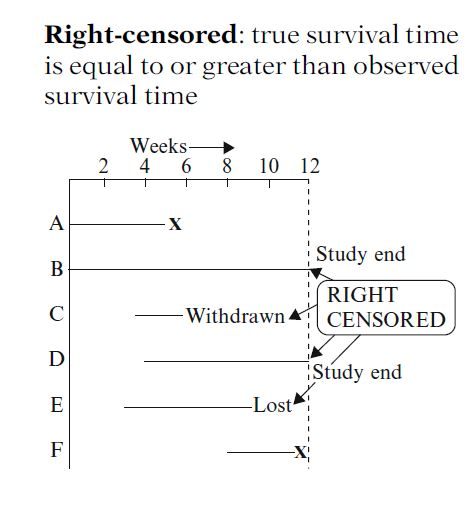
\includegraphics[width = \textwidth]{Ch1-RightCensor.JPG}
%    \end{column}
%    \hspace{-40pt}
%    \begin{column}{0.48\textwidth}
%         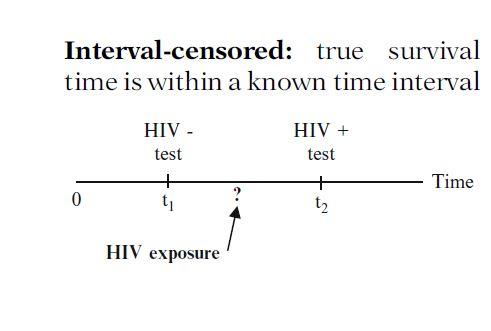
\includegraphics[width = \textwidth]{Ch1-IntervalCensor.JPG} \\
%              \vspace{-20pt}
%         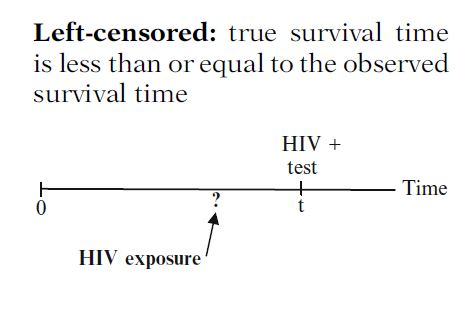
\includegraphics[width =\textwidth]{Ch1-LeftCensor.JPG}
%    \end{column}
%\end{columns}
%\end{frame}
%\begin{frame} \frametitle{Considerations about hazard rate}
%\begin{block}{Hazard rate is dependent on time}
%\begin{enumerate}
%\item The hazard rate is dependent on the unit of measurement of time. For example, say $S$ is time measured in seconds.
%\[
%h(s) = \lim_{\Delta s \to 0} \frac{P(S + \Delta s|S \ge s)}{\Delta s}
%\]
%
%If say, $T$ is time measure in minutes then
%\begin{align*}
%h(t) & = \lim_{\Delta t \to 0} \frac{P( + \Delta t|S \ge t)}{\Delta t} \\
%& = \lim_{\Delta s \to 0} \frac{P(T/60 + \Delta t/60| T/60 \ge t/60)}{ \Delta t/60} = 60 h(s)
%\end{align*}
%
%\end{enumerate}
%\end{block}
%\end{frame}
%
%\begin{frame}\frametitle{Considerations about hazard rate (cont'd)}
%\begin{block}{Other considerations about hazard rate}
%\begin{enumerate}
%  \setcounter{enumi}{1}
%\item Relative rates of hazard are the same at any particular time.  For example, at any particular time (in seconds),~$s$, let $h(s,0)$ be the hazard for men (sex=0) and $h(s,1)$ be the hazard for women (sex=1). Then with $t$ the time in minutes,
%    \[ \dfrac{h(t,0)}{h(t,1)} =  \dfrac{60 h(s,0)}{60 h(s,1)} = \dfrac{ h(s,0)}{ h(s,1)}
%    \]
%\item Can identify underlying distribution from hazard rate, for example, exponential has constant hazard, Weibull has proportional and monotonic hazard, lognormal has increasing than decreasing hazard, etc.
%\item Can recover survival function from hazard rate.
%\end{enumerate}
%\end{block}
%\end{frame}
%
%\begin{frame}\frametitle{Hazard Functions of Different Distributions}
%\begin{columns}
%    \begin{column}{0.48\textwidth}
%        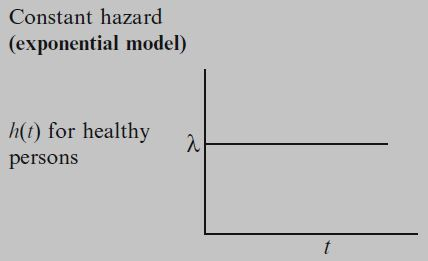
\includegraphics[width = \textwidth]{Hazards1.JPG} \\
%           \includegraphics[width = \textwidth]{Hazards2.JPG}
%    \end{column}
%    \hspace{-10pt}
%    \begin{column}{0.48\textwidth}
%              \vspace{-20pt}
%         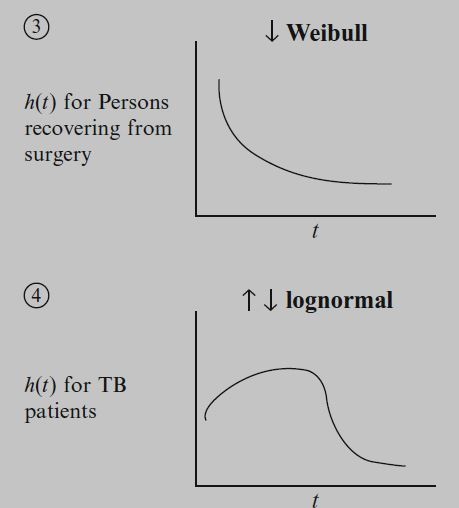
\includegraphics[width =\textwidth]{Hazards3.JPG}
%    \end{column}
%\end{columns}
%\end{frame}
%
%
%
%\begin{frame}
%\frametitle{Ways to represent (right censored) survival data (cont'd)}
%\begin{block}{First way to represent data }
%\begin{columns}
%    \begin{column}{0.48\textwidth}
%        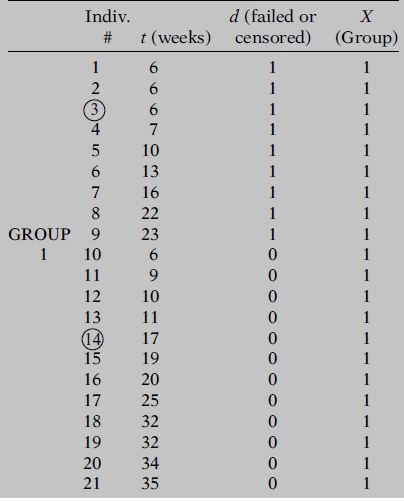
\includegraphics[width =\textwidth, height=6cm]{Ch1-leuk_dat_a.JPG}
%    \end{column}
%    \hspace{-10pt}
%    \begin{column}{0.48\textwidth}
%         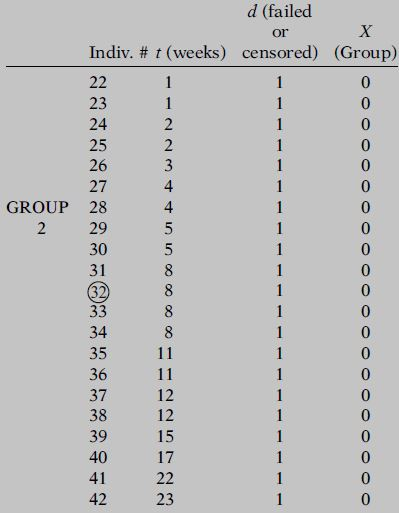
\includegraphics[width =\textwidth, height=6cm]{Ch1-leuk_dat_b.JPG}
%    \end{column}
%\end{columns}
%\end{block}
%\end{frame}
%
%\begin{frame}
%\frametitle{Ways to represent (right censored) survival data}
%Consider the following data of times to remission of leukemia patients:
%\begin{block}{Second way to represent data }
%\begin{table}
%\begin{center}
%\begin{tabular}{l l}
%Group 1 (n=21) treatment & Group 2 (n=21) placebo \\
% 6, 6, 6, 7, 10, 13, 16, 22, 23, & 1, 1, 2, 2, 3, 4, 4, 5, 5,  \\
% 6+, 9+, 10+, 11+, 17+, 19+, & 8, 8, 8, 8, 11, 11, 12, 12, \\
%   20+, 25+, 32+, 32+, 34+, 35+ & 15, 17, 22, 23
%\end{tabular}
%\end{center}
%\end{table}
%Note: + denotes censored
%\end{block}
%\end{frame}
%
%\begin{frame}
%\frametitle{Ways to represent (right censored) survival data (cont'd)}
%\begin{block}{Third way to represent data }
%\begin{columns}
%    \begin{column}{0.48\textwidth}
%        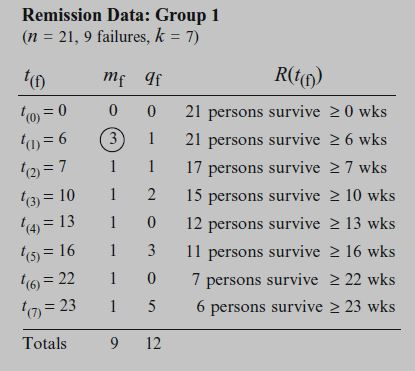
\includegraphics[width =\textwidth, height=6cm]{Ch1-leuk_data_a1.JPG}
%    \end{column}
%    \hspace{-10pt}
%    \begin{column}{0.48\textwidth}
%         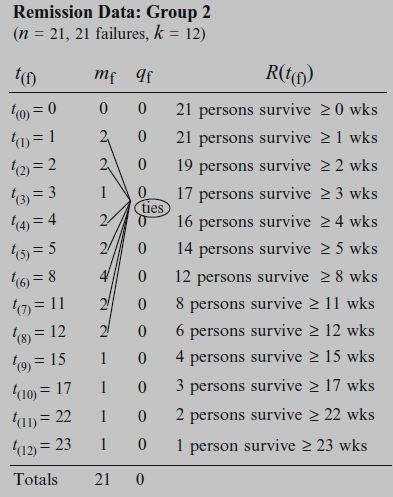
\includegraphics[width =\textwidth, height=6cm]{Ch1-leuk_data_b1.JPG}
%    \end{column}
%\end{columns}
%\end{block}
%\end{frame}
%
%\begin{frame}
%\frametitle{Ways to represent (right censored) survival data (cont'd)}
%\begin{block}{Fourth way to represent data - Counting Process (CP) format}
%\begin{columns}
%    \begin{column}{0.48\textwidth}
%        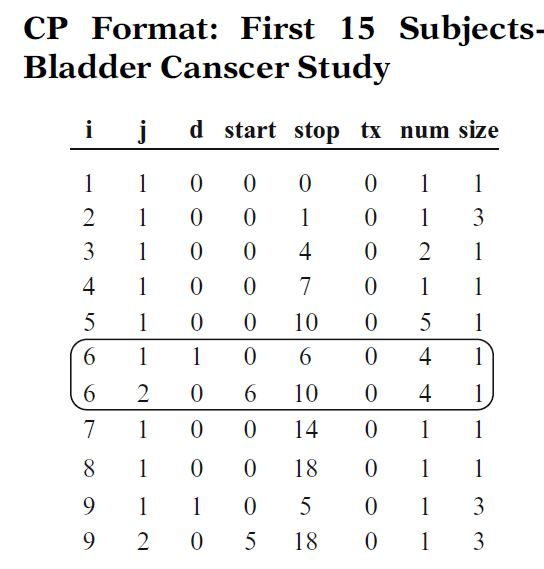
\includegraphics[width =\textwidth, height=5.5cm]{Ch1-CPFormat_1.JPG}
%    \end{column}
%    \hspace{-10pt}
%    \begin{column}{0.48\textwidth}
%         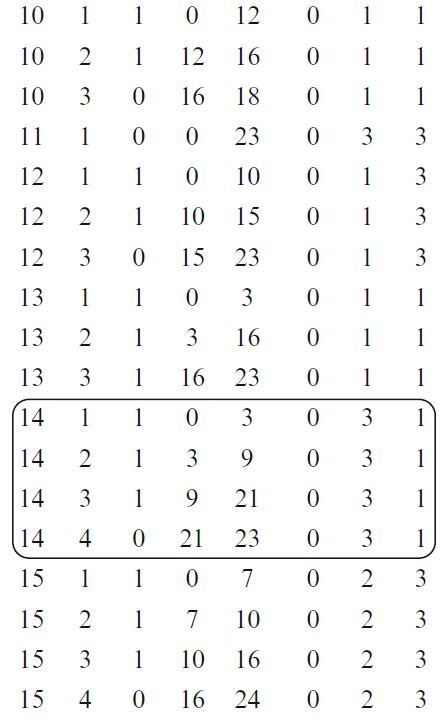
\includegraphics[width =\textwidth, height=5.5cm]{Ch1-CPFormat_2.JPG}
%    \end{column}
%\end{columns}
%\end{block}
%\end{frame}
%
%\begin{frame}
%\frametitle{Ways to represent (right censored) survival data (cont'd)}
%\begin{block}{Fourth way to represent data }
%\begin{itemize}
%\item This data is the the recurrence of bladder cancer tumors after transurethral surgical excision.
%\item Covariates are tx (0 or 1), num and size. Only tx=0 is included here.
%\item $i$ is the subject, $j$ is the number of the event for the subject.
%\item $d$ is censoring status, \textbf{start} is when event starts, \textbf{stop} is last time of observation of event.
%\item For subject 6, two events are observed.
%\begin{enumerate}[i.]
%\item The first tumor starts at time 0 and stops (excised) at time 6.
%\item The second tumor starts at time 6 and the observation is censored at time 10.
%\end{enumerate}
%\end{itemize}
%\end{block}
%\end{frame}
%
%\begin{frame}
%\frametitle{Kaplan Meier Estimates of Survival}
% 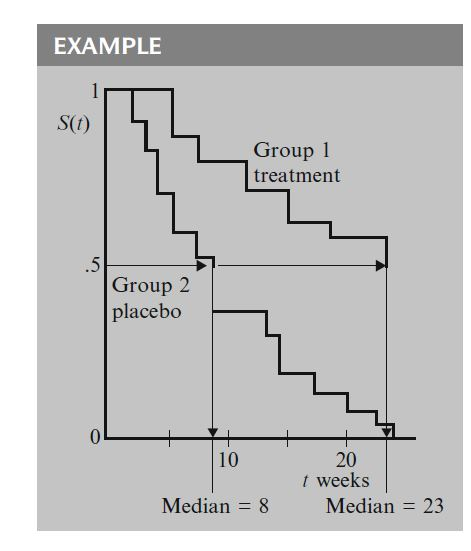
\includegraphics[width =\textwidth, height=5.5cm]{Ch1_estsurv.JPG}
% \end{frame}
%
%\begin{frame}
%\frametitle{Remission Data with LogWBC (Confounding Example)}
% 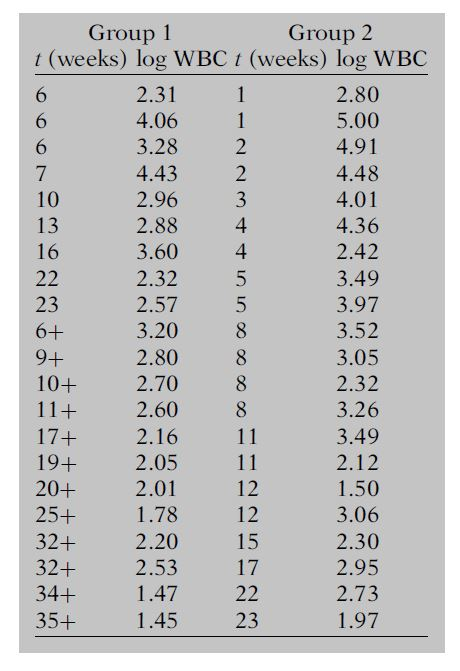
\includegraphics[width =\textwidth, height=6.5cm]{Ch1-RemissionwLogwbc.JPG}
% \end{frame}
%
%\begin{frame}
%\frametitle{Confounding Example}
% 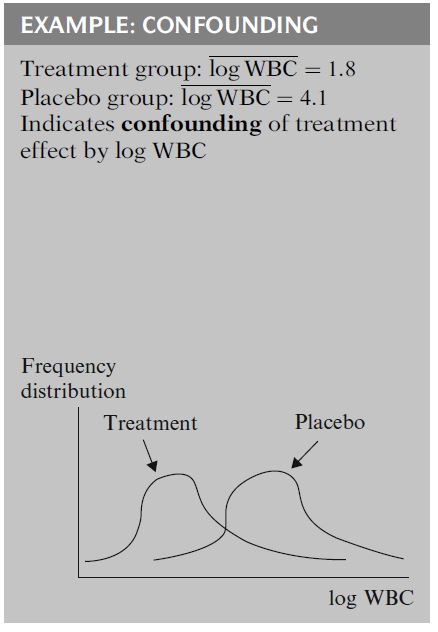
\includegraphics[width =\textwidth, height=6.5cm]{Ch1_Confound.JPG}
% \end{frame}
%
%\begin{frame}
%\begin{block}{Remark 1.4 - Confounding}
%\begin{itemize}
%\item We see the distribution of logWBC for the Treatment group and for the Placebo group.
%\item The Placebo group tends to have higher logWBC with the mean logWBC for Treatment of 1.8 and the the mean logWBC for Placebo of 4.1.
%\item Thus, if lower logWBC correlates with greater survival times, the effect of the treatment in creating greater survival times might be from this correlation rather than the effect of the treatment in itself.
%\item In this case, the effect of treatment is \textbf{confounded} by the effect of treatment.
%\item Confounding is dealt with by including secondary variables in semi-parametric models and parametric models.
%\end{itemize}
%\end{block}
%\end{frame}
%
%
%\begin{frame}
%\frametitle{Interaction Example}
% 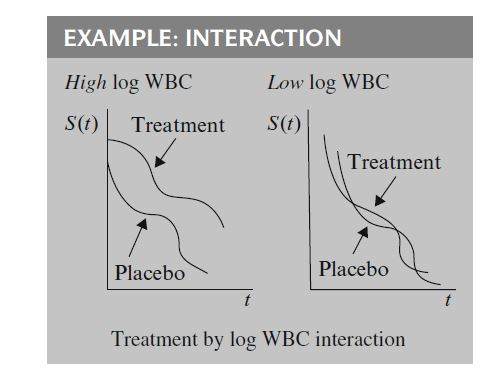
\includegraphics[width =\textwidth, height=6.5cm]{Ch1_Interact.JPG}
% \end{frame}
%
%
%\begin{frame}
%\begin{block}{Remark 1.4 - Interaction}
%\begin{itemize}
%\item We see the affect of Treatment depends on the level of logWBC.
%\item For high logWBC Treatment has a positive effect on survival probabilities.
%\item For low logWBC Treatment does not have a significant effect on survival probabilities.
%\item Interaction is dealt with by 1) partitioning data on different levels of the secondary variable or 2) by including interaction terms in semi-parametric and parametric models.
%\end{itemize}
%\end{block}
%\end{frame}
%
%
%\begin{frame}
%\frametitle{Assumptions about (right) censoring}
%\begin{block}{Definition 1.9 - Random Censoring and Independent Censoring}
%\begin{itemize}
%\item \textbf{Random censoring} means that subjects who are censored at
%time $t$ are representative of all the study subjects who remained at risk at time $t$ with respect to their survival experience. Thus, the failure rate for subjects who are
%censored is assumed to be equal to the failure rate for subjects who remained in the risk set who are not censored.
%\item \textbf{Independent censoring} means within any subgroup of interest, the subjects who are censored at time $t$ should be representative of all the subjects in that subgroup who remained at risk at time $t$ with respect to their survival experience. Thus, censoring is independent provided that it is random within any subgroup of interest.
%\end{itemize}
%\end{block}
%\end{frame}
%
%
%
%\begin{frame}
%\frametitle{Assumptions about censoring}
%\begin{block}{Example 1.1}
%Consider a population with two groups - Group A and Group B.
%\begin{center}
%\textbf{Group A}
%\begin{tabular}{ c c c c }
% Time & \# at risk & \# events & \# survived \\ \hline
% 0-3 yrs & 100 & 20 & 80 \\
% 3–5 yrs &  40 & 5 & 35
%\end{tabular} \\
%40 left study at the end of 3 years
%\end{center}
%\begin{center}
%\textbf{Group B}
%\begin{tabular}{ c c c c }
% Time & \# at risk & \# events & \# survived \\ \hline
% 0-3 yrs & 100 & 40 & 60 \\
% 3–5 yrs &  50 & 10 & 40
%\end{tabular} \\
%10 left study at the end of 3 years.
%\end{center}
%\end{block}
%Assuming, independent censoring summarize the 3 and 5 year survival experiences of both groups.
%\end{frame}
%
%\begin{frame}
%\frametitle{Assumptions about censoring (cont'd)}
%\begin{block}{Example 1.1}
%Consider the entire population.
%\begin{center}
%\textbf{All}
%\begin{tabular}{ c c c c }
% Time & \# at risk & \# events & \# survived \\ \hline
% 0-3 yrs & 200 & 60 & 140 \\
% 3–5 yrs &  90 & 15 & 75
%\end{tabular} \\
%50 left study at the end of 3 years.
%\end{center}
%\end{block}
%If we assume independent censoring, do we have random censoring?
%\end{frame}
%
%\begin{frame}
%\frametitle{Assumptions about censoring (cont'd)}
%\begin{block}{Remark 1.4 - Random vs. Independent Censoring}
%\begin{itemize}
%\item Random censoring is a stronger condition than independent censoring.
%\item Independent censoring only applies to groups of interest and random censoring applies to every subgroup including the entire data set.
%\item Independent censoring is random censoring conditional on each level of covariates.
%\item We only need and assume independent censoring for our covariates of interest.
%\end{itemize}
%\end{block}
%\end{frame}
%
%
%\begin{frame}
%\frametitle{Assumptions about censoring (cont'd)}
%\begin{block}{Remark 1.5 - Informative vs. NonInformative Censoring}
%\begin{itemize}
%\item \textbf{ Non-informative censoring} occurs if the distribution of survival times ($T$) provides no
%information about the distribution of censorship times ($C$), and vice versa. Otherwise, the
%censoring is \textbf{informative}.
%\item Independent censoring commonly fails when there is a drug side-effect that causes patients to drop out. In this case, those in the treatment group are not being censored at ``random'' and if we assume independent censoring then we are overestimating the survival experience of the treatment group. We assume independent censoring in this course.
%\end{itemize}
%\end{block}
%\end{frame}


%\section{Chapter 2}
%
%\begin{frame}
%\frametitle{Constructing Kaplan-Meirer Curves}
%Consider the following data (from chapter 1) of times to remission of leukemia patients:
%\begin{block}{Remission Data }
%\begin{table}
%\begin{center}
%\begin{tabular}{l l}
%Group 1 (n=21) treatment & Group 2 (n=22) placebo \\
% 6, 6, 6, 7, 10, 13, 16, 22, 23, & 1, 1, 2, 2, 3, 4, 4, 5, 5,  \\
% 6+, 9+, 10+, 11+, 17+, 19+, & 8, 8, 8, 8, 11, 11, 12, 12, \\
%   20+, 25+, 32+, 32+, 34+, 35+ & 15, 17, 22, 23
%\end{tabular}
%\end{center}
%\end{table}
%Note: + denotes censored
%\end{block}
%\end{frame}
%
%\begin{frame}
%\frametitle{Constructing Kaplan-Meirer Curves (cont'd)}
%\begin{block}{Remission Data (another way)}
%\begin{columns}
%    \begin{column}{0.48\textwidth}
%        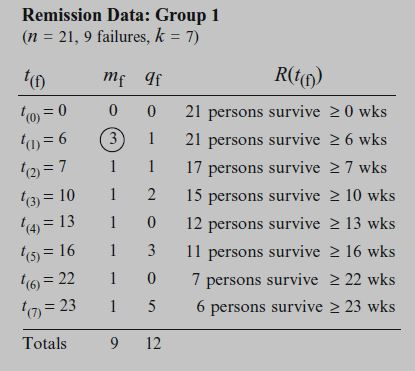
\includegraphics[width =\textwidth, height=6cm]{Ch1-leuk_data_a1.JPG}
%    \end{column}
%    \hspace{-10pt}
%    \begin{column}{0.48\textwidth}
%         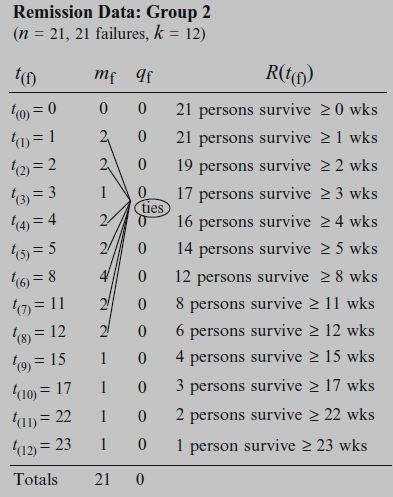
\includegraphics[width =\textwidth, height=6cm]{Ch1-leuk_data_b1.JPG}
%    \end{column}
%\end{columns}
%\end{block}
%\end{frame}
%
%
%\begin{frame}
%\frametitle{Constructing Kaplan-Meirer Curves (cont'd)}
%\begin{block}{Kaplan-Meirer Estimates for Group 2}
%\begin{columns}
%    \begin{column}{0.48\textwidth}
%        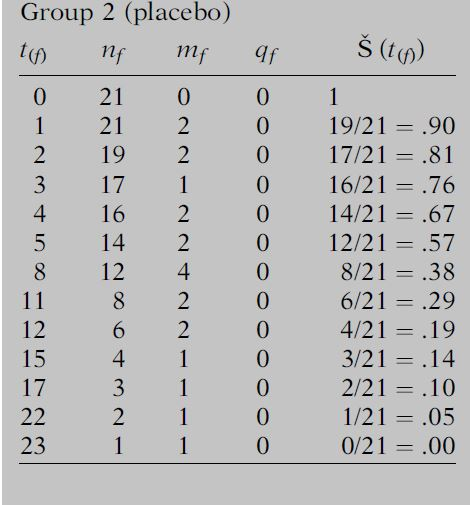
\includegraphics[width =\textwidth, height=5.5cm]{Ch2_KMGP2.JPG}
%    \end{column}
%    \hspace{-10pt}
%    \begin{column}{0.48\textwidth}
%         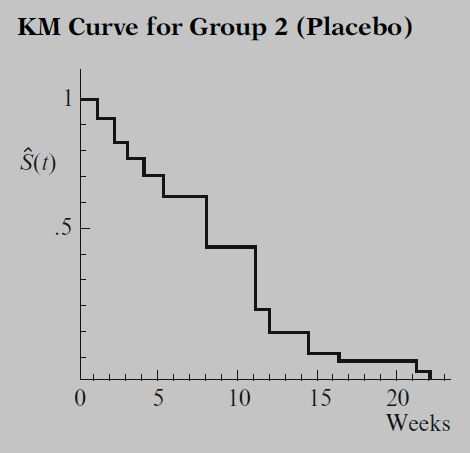
\includegraphics[width =\textwidth, height=5.5cm]{Ch2_KMCGP2.JPG}
%    \end{column}
%\end{columns}
%\end{block}
%\end{frame}
%
%\begin{frame}
%\frametitle{Constructing Kaplan-Meirer Curves (cont'd)}
%\begin{block}{Problem 2.1 - Kaplan-Meirer Estimates for Group 1}
%         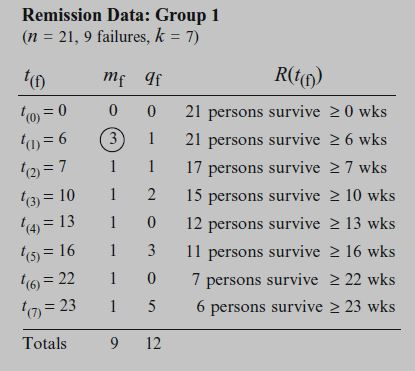
\includegraphics[width =\textwidth, height=5.5cm]{Ch1-leuk_data_a1.JPG}
%\end{block}
%Find the Kaplan-Meirer Estimates for Group 1 and plot the Kaplan-Meirer Curves for groups 1 and 2.
%\end{frame}
%
%\begin{frame}
%\frametitle{Constructing Kaplan-Meirer Curves (cont'd)}
%\begin{block}{Kaplan-Meirer Curves for Groups 1 and 2}
%         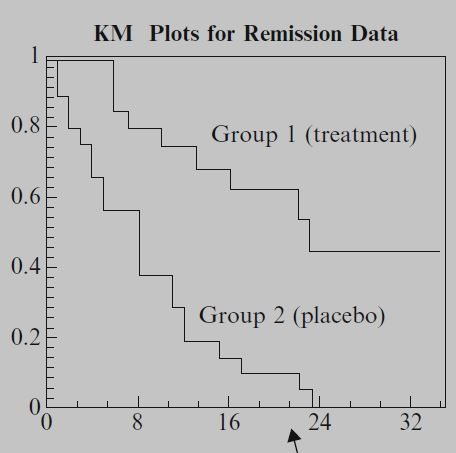
\includegraphics[width =\textwidth, height=5.5cm]{Ch2_KM_GR12.JPG}
%\end{block}
%\end{frame}
%
%\begin{frame}
%\frametitle{Constructing Kaplan-Meirer Curves (cont'd)}
%\begin{block}{Problem 2.2 - Kaplan-Meirer Estimates in R}
%\begin{enumerate}
%\item Find the KM Estimates for the entire remission data set in R
%\item Plot the KM curve for the entire remission data set in R
%\item Find the KM Estimates for group 1 and group 2 in R
%\item For groups 1 and 2 and plot the KM Curves for Groups 1 and 2 in R
%\end{enumerate}
%\end{block}
%\end{frame}
%
%\begin{frame}
%\frametitle{Log-Rank Tests for Survival Experiences}
%\begin{block}{Log-Rank Tests for two groups}
%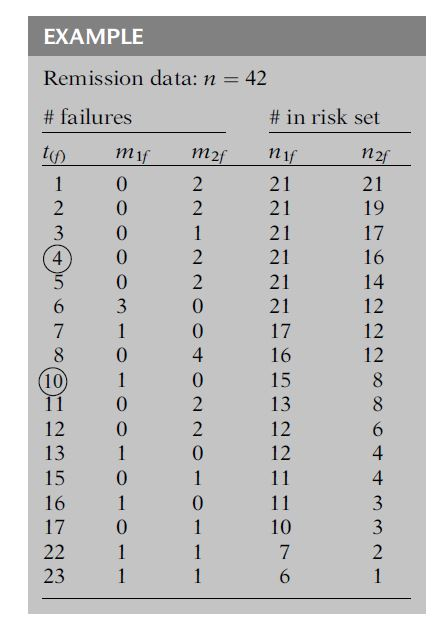
\includegraphics[width =\textwidth, height=5.5cm]{CH2_LogRank.JPG}
%\end{block}
%\end{frame}
%
%\begin{frame}
%\frametitle{Log-Rank Tests for Survival Experiences (cont'd)}
%\begin{block}{Log-Rank test for two groups}
%We can test whether the null hypothesis, $H_0$, that the survival experiences for these two groups is the same as follows.
%\begin{enumerate}
%\item Find the \textbf{expected cell counts}.
%\begin{align*}
%e_{1f} & = \left(\frac{n_{1f}}{n_{1f} + n_{2f}}\right)(m_{1f} + m_{2f}) \\
%e_{2f} & = \left(\frac{n_{2f}}{n_{2f} + n_{2f}}\right)(m_{1f} + m_{2f})
%\end{align*}
%\end{enumerate}
%\end{block}
%\end{frame}
%
%\begin{frame}
%\frametitle{Log-Rank Tests for Survival Experiences (cont'd)}
%\begin{block}{Log-Rank test for two groups (cont'd)}
%
%\begin{enumerate}
% \setcounter{enumi}{1}
%\item Find the total number of observed minus expected failures
%\[
%O_i - E_i = \sum_{i=1}^k (m_{if} - e_{if}), \, i=1,2
%\]
%Where $k$ is total number of events. \\
%We must have $O_1 - E_1 = -(O_2- E_2)$.
%\end{enumerate}
%\end{block}
%\end{frame}
%
%\begin{frame}
%\frametitle{Log-Rank Tests for Survival Experiences (cont'd)}
%\begin{block}{Log-Rank test for two groups (cont'd)}
% \begin{enumerate}
%  \setcounter{enumi}{2}
%\item Form the log rank statistic
%\[
%LRS = \frac{(O_i - E_i)^2}{\text{Var}(O_i-E_i)} \text{ for } i=1 \text{ or } i=2
%\]
%or approximate LRS
%\[
%LRS = \sum_i^{2} \frac{(O_i - E_i)^2}{E_i}
%\]
%\item Reject $H_0$ iff $\text{LRS} > \chi^2_{\alpha,1}$ where $\alpha$ is the significance of test or
%\[
%\text{p-value} = P(X>LRS), \,  X \sim \chi^2_1 \text{ reject iff p-value} \le \alpha.
%\]
%\end{enumerate}
%\end{block}
%\end{frame}
%
%\begin{frame}
%\frametitle{Log-Rank Tests for Survival Experiences (cont'd)}
%\begin{block}{Log-Rank test for two groups (cont'd) - Remission Data}
%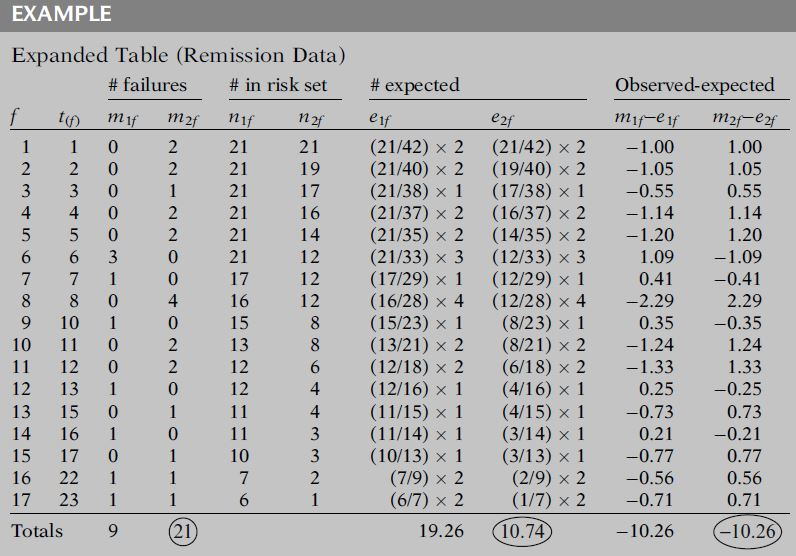
\includegraphics[width =\textwidth, height=5.5cm]{CH2_ComputeLR}
%\end{block}
%\end{frame}
%
%
%\begin{frame}
%\frametitle{Log-Rank Tests for Survival Experiences (cont'd)}
%\begin{block}{Log-Rank test for $G>2$ groups}
%The null hypothesis, $H_0$, is that the survival experiences for \textit{all} groups is the same.
%\begin{enumerate}
%\item Find the \textbf{expected cell counts}.
%\begin{align*}
%e_{if} & = \left(\frac{n_{if}}{n_{f}}\right)(m_{f}) \\
%n_{f} & = \sum_{i=1}^G n_{if}, \, m_f =  \sum_{i=1}^G m_{if}\\
%\end{align*}
%where $n_{if}=$\# at risk at $t_f$ for group $i$, \, $m_{if}=$\# of failures at $t_f$ for group $i$.
%\end{enumerate}
%\end{block}
%\end{frame}
%
%\begin{frame}
%\frametitle{Log-Rank Tests for Survival Experiences (cont'd)}
%\begin{block}{Log-Rank test for $G>2$ groups}
%\begin{enumerate}
% \setcounter{enumi}{1}
%\item Find the total number of observed minus expected failures
%\[
%O_i - E_i = \sum_{i=1}^k (m_{if} - e_{if}), \, i=1,2, \ldots, G.
%\]
%where $k$ is total number of events.
%\item Find approximate log-rank statistic
%\[
%LRS = \sum_i^{\text{\# groups}} \frac{(O_i - E_i)^2}{E_i}
%\]
%Exact LRS is given in Chapter 2 appendix.
%\end{enumerate}
%\end{block}
%\end{frame}
%
%\begin{frame}
%\frametitle{Log-Rank Tests for Survival Experiences (cont'd)}
%\begin{block}{Log-Rank test for $G>2$ groups}
%\begin{enumerate}
%\setcounter{enumi}{3}
%\item Reject $H_0$ iff $\text{LRS} > \chi^2_{\alpha,G-1}$ where $\alpha$ is significance of test or
%\[
%\text{p-value} = P(X>LRS), \,  X \sim \chi^2_{G-1} \text{ reject iff p-value} \le \alpha.
%\]
%\end{enumerate}
%\end{block}
%\begin{block}{Vets data set}
%Vets.dat reports on survival times in days for 137 patients from the Veteran’s Administration Lung Cancer Trial:
%\begin{center}
%\includegraphics[width =4.5cm, height=3.5cm]{CH2_Vets}
%\end{center}
%\end{block}
%\end{frame}
%\begin{frame}
%\frametitle{Log-Rank Tests for Survival Experiences (cont'd)}
%\begin{block}{Problem 2.3 - Log-Rank Tests in R}
%\begin{enumerate}
%\item In R conduct a Log-Rank test for the two groups in the Remission Data. What conclusion do you reach?
%\item In R conduct partition the Vets.dat data set into three groups by Performance Status: Group 1: 0-59, Group 2: 60-74 and Group 3: 75-100. Create and plot KM estimates for these three groups and conduct an overall log-rank test to test if the survival experiences are the same. What conclusion do you reach?
%\end{enumerate}
%\end{block}
%\end{frame}
%\begin{frame}
%\frametitle{Variations and Extensions of the Log-Rank Test}
%\begin{block}{Alternative Log-Rank Tests}
%The Wilcoxon, Tarone-Ware, Peto and Flemington-Harrington tests work by weighting observed - expected numbers of events. That is, they weight terms in the log rank test
%\[
%O_i - E_i = \sum_f (m_{if}-e_{if}) \text{ to get } \sum_f w(t_{(f)})(m_{if}-e_{if})
%\]
%and use test statistic
%\[
%\frac{\left(\sum_f w(t_{(f)}) (m_{if}-e_{if})\right)^2}{var(w(t_{(f)}) (m_{if}-e_{if}))}.
%\]
%\end{block}
%\end{frame}
%
%\begin{frame}
%\frametitle{Variations and Extensions of the Log-Rank Test (cont'd)}
%\begin{block}{Alternative Log-Rank Tests (cont'd)}
%We look at the Flemington-Harrington test. This test uses weights
%\[ w(t_{(f)}) = (\hat{S}(t_{(f-1)}))^p (1-\hat{S}(t_{(f-1)}))^q \text{ with } p,q \ge 0.
%\]
%
%\begin{itemize}
%\item If $p=q=0$ then we recover the log rank test.
%\item If $q=0, p>0$ as $\hat{S}(t_{(f-1)})^p $ is a decreasing (non-increasing) function of $f$, earlier times are going to weigh more heavily in determining differences than later times.
%\item If $p=0, q>0$ as $(1-\hat{S}(t_{(f-1)})^q $ is an increasing (non-decreasing) function of $f$, earlier times are going to weigh less heavily in determining differences than later times.
%\item Given $q=0$ how differences are weighed can be determined by examining the function $x^p$ for various $p>0$.
%\end{itemize}
%\end{block}
%\end{frame}
%
%\begin{frame}
%\frametitle{Variations and Extensions of the Log-Rank Test (cont'd)}
%\begin{block}{Alternative Log-Rank Tests (cont'd)}
%Assume in the Flemington-Harrington test $q=0$. For $p=3$ the importance of earlier times falls off quickly and then flattens. For $p=0.15$ the importance of early times decreases slowly then falls off quickly at the end.
%\begin{center}
%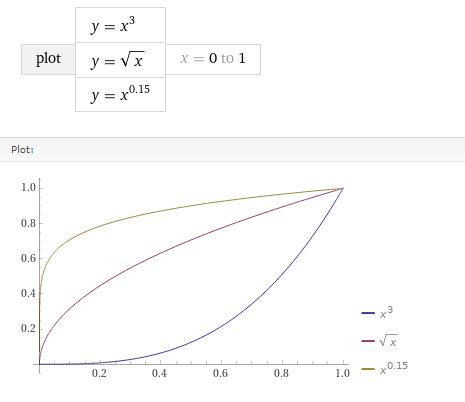
\includegraphics[width =4.5cm, height=3.5cm]{Ch2_Flemharringtonplot.JPG}
%\end{center}
%\end{block}
%\end{frame}
%
%\begin{frame}
%\frametitle{Variations and Extensions of the Log-Rank Test (cont'd)}
%\begin{block}{Problem 2.4 - Alternative Log-Rank Tests (cont'd)}
%Conduct the Flemington-Harrington Test in R with $q=0$ and $p=0, 0.15, 0.5$ and 3 to compare the Placebo vs. Treatment groups in the remission data. Considering the Kaplan-Meirer estimates below, what should happen to the Chi-Square statistic as $p$ increases?
%\end{block}
%\begin{center}
%         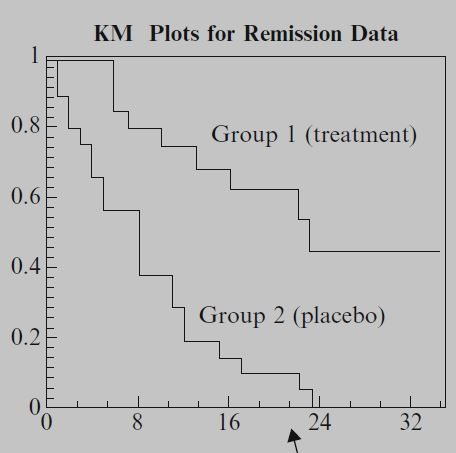
\includegraphics[width =5.0cm, height=4.0cm]{Ch2_KM_GR12.JPG}
%\end{center}
%\end{frame}
%
%\begin{frame}
%\frametitle{Variations and Extensions of the Log-Rank Test (cont'd)}
%\begin{block}{The stratified log rank test}
%If there is confounding, then the log rank test with respect to the exposure variable can be misleading. Instead, we can stratify on the confounding variable, compute observed and expected number of events at each time across strata.
%\[
%O_i-E_i = \sum_s \sum_f (m_{ifs} - e_{ifs})
%\]
%where $i=$ group, $f=$failure time, $s=$stratum.
%Then we compute test statistic
%\[ \sum_{i=1}^{G-1} \frac{O_i-E_i}{var(O_i-E_i)}
%\]
%\end{block}
%\end{frame}
%
%\begin{frame}
%\frametitle{Variations and Extensions of the Log-Rank Test (cont'd)}
%\begin{block}{The stratified log rank test - Remission Data}
%LogWbc is a possible confounder.
%\begin{center}
%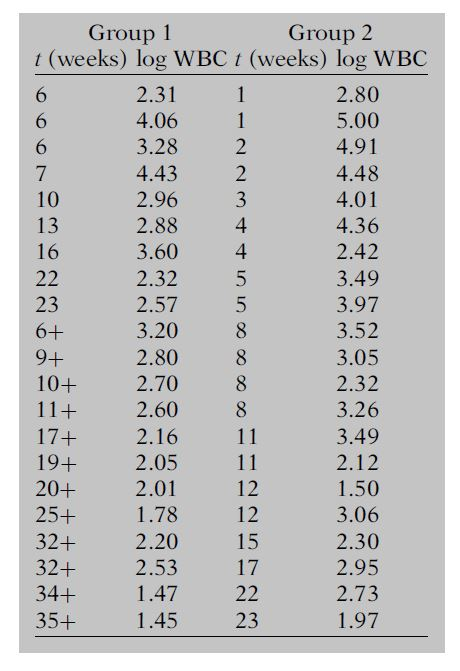
\includegraphics[width =4.5cm, height=5cm]{Ch1-RemissionwLogwbc.JPG}
%\end{center}
%\end{block}
%\end{frame}
%
%\begin{frame}
%\frametitle{Variations and Extensions of the Log-Rank Test (cont'd)}
%\begin{block}{The stratified log rank test - Remission Data}
%We statify on LogWbc with low (1) - 1.45 to 2.30, \\ med (2) - 2.31 to 3.00, high (3) 3.01 to 5.00 and compute:
%\begin{columns}
%    \begin{column}{0.48\textwidth}
%        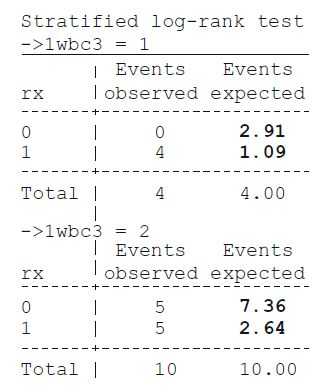
\includegraphics[width =\textwidth, height=5.5cm]{strat_lr1.JPG}
%    \end{column}
%    \hspace{-10pt}
%    \begin{column}{0.48\textwidth}
%         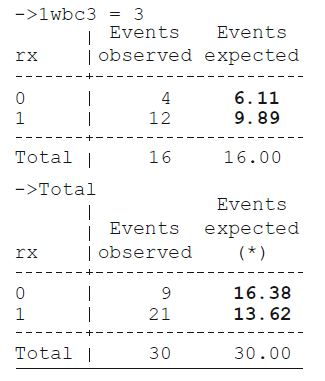
\includegraphics[width =\textwidth, height=5.5cm]{strat_lr2.JPG}
%    \end{column}
%\end{columns}
%\end{block}
%\end{frame}
%
%\begin{frame}
%\frametitle{Variations and Extensions of the Log-Rank Test (cont'd)}
%\begin{block}{Problem 2.5: The stratified log rank test - Remission Data}
%\begin{enumerate}
%\item Confirm the computations in the previous slide in the first strata (1.50-2.30) of LogWBC.
%\item Compute the stratified log rank statistic in R.
%\item Make a conclusion about your test and find a $p$-value.
%\end{enumerate}
%\end{block}
%\end{frame}
%
%\begin{frame}
%\frametitle{Confidence Intervals about KM estimates}
%\begin{block}{Greenwood's formula for SE of estimated survival probabilities}
%A 100$(1-\alpha)\%$ CI for the estimated KM survival estimates:
%\[
%\hat{S}_{KM}(t) \pm z_{\alpha/2}\text{SE}({S}_{KM}(t))
%\]
%where $\text{SE}(\hat{S}_{KM}(t)) = \sqrt{\hat{Var}[\hat{S}_{KM}(t)]}.$
%\textbf{By Greenwood's formula}
%\[
%\hat{Var}[\hat{S}_{KM}(t)] = (\hat{S}_{KM}(t))^2 \sum_{f:t_{(f)} \le t}\left[\frac{m_f}{n_f(n_f-m_f)}\right]
%\]
%\end{block}
%\end{frame}
%
%\begin{frame}
%\frametitle{Confidence Intervals about KM estimates}
%\begin{block}{Greenwood's formula for SE of estimated survival probabilities (cont'd)}
%\textbf{Greenwood's formula} applied to treatment group in the Remission data
%\begin{center}
%   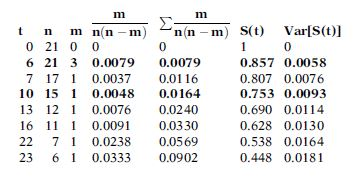
\includegraphics[width =6cm, height=4cm]{Ch2_Greenwoods.JPG}
%\end{center}
%\end{block}
%\end{frame}
%
%\begin{frame}
%\frametitle{Confidence Intervals about KM estimates}
%\begin{block}{Problem 2.6 - Confidence Intervals for KM estimates}
%\begin{enumerate}
%\item Find confidence intervals about KM estimates at times 6 and 7 for the treatment group using the above table.
%\item Use R to find confidence intervals about the KM estimates for the treatment group.
%\item Use R to plot the survival curves and confidence bands for the treatment and placebo groups.
%\end{enumerate}
%\end{block}
%\end{frame}
%  %
%\begin{frame}
%\frametitle{Confidence Interval for the median}
%\begin{block}{Large sample confidence interval for $M$}
%We use the large sample distribution
%\[ \frac{\hat{S}_{KM}(M) - 0.5}{\hat{SE}[\hat{S}_{KM}(M)]} \sim Z \text{ where } Z \sim N(0,1) \text { and } M \text{ is the median.}
%\]
%Thus, we have
%\begin{align*}
%&P(0.5 - z_{\alpha/2}\hat{SE}[\hat{S}_{KM}(M)] <  \hat{S}_{KM}(M) < 0.5 + z_{\alpha/2}\hat{SE}[\hat{S}_{KM}(M)]) \\
%&\approx 1-\alpha
%\end{align*}
%and it is reasonable to take a $1-\alpha$ C.I. for $M$ as all $M$ that satisfy the above inequality. Often, the half open interval to the survival times one above the largest $M$'s that satisfies this inequality is used.
%\end{block}
%\end{frame}
%
%
%\begin{frame}
%\frametitle{Confidence Interval for the median}
%\begin{block}{Problem 2.6 - Large sample confidence interval for $M$}
%Use R to find a $95\%$ confidence interval for the median for the placebo and survival groups for the Remission data.
%\end{block}
%\end{frame}


\section{Chapter 3}

\begin{frame}
\frametitle{The Cox Proportional Hazard Model}
\begin{block}{Definition 3.1 - Form of the Cox Proportional Hazard (PH) Model}
Let $h$ be the hazard function of a survival population. If the Cox PH assumption is satisfied then
\[
h(t,\mathbf(X)) = h_0(t)\exp\left(\sum_{i=1}^p \beta_i X_i\right) = h_0(t)\exp(\beta X')
\]
for some fixed parameters $\beta=(\beta_1,\ldots,\beta_p)$, for any $t>0$ of interest and for any covariates specified as $X=(X_1,\ldots,X_p)$. The function $h_0(t)$ is known as the \textbf{baseline hazard function}.
\end{block}
\end{frame}

\begin{frame}
\frametitle{The Cox Proportional Hazard Model, cont'd}
\begin{block}{Remark 3.1 - Implications of Cox PH assumption}
\begin{enumerate}
\item The proportional hazards assumption is satisfied (see Theorem 3.1)
\item Provided there is not interaction with another covariate, the effect on the hazard ratio of a unit increase in a covariate $X_i$ is $\exp(\beta_i)$.
\item The covariates should be \textbf{time-independent} else the PH assumption will not be met.
\end{enumerate}
\end{block}
\end{frame}

\begin{frame}
\frametitle{The Cox Proportional Hazard Model, cont'd}
\begin{block}{Remark 3.2 - Interaction terms}
\begin{enumerate}
\item We defined interaction in \idf{1.8} as ``when the effect of the change in a variable on survival probabilities depends on the level of a secondary variable''.
\item One way we can account for interaction between two covariates ($X_i$ and $X_j$  with $i \neq j$) in a semi- or fully parametric model is by including an interaction term $\alpha X_iX_j$.
\item Assuming $\beta X_i$ in the model and no other interaction terms besides $\beta_j X_i X_j$ are in the model, the effect of a unit increase of $X_i$ on the hazard rate in a Cox PH model is
\[
\exp(\beta_i + \beta_j X_j)
\]
which depends on $X_2$ (hence the interaction).
\end{enumerate}
\end{block}
\end{frame}

\begin{frame}
\frametitle{The Cox Proportional Hazard Model, cont'd}
\begin{block}{Problem 3.1 - Cox PH Model for the Remission Data}
\begin{enumerate}
\item In R, build three Cox PH models for the Remission data:
\begin{enumerate}[i]
\item A model that just accounts for treatment status (TR)
\item A model that accounts for TR and logWBC
\item A model that accounts for interaction between TR and logWBC
\end{enumerate}
\item Interpret the coefficients of the models, find confidence intervals for the coefficients and changes in HR and test the significance of the coefficients.
\item Choose the "best" model based on your last answer.
\end{enumerate}
\end{block}
\end{frame}

\begin{frame}
\frametitle{The Cox Proportional Hazard Model, cont'd}
\begin{block}{Remark 3.1 - Model Selection and Parsimony}
Why not include the interaction term? Even though the interaction effect is ``small'' won't this give us a better idea of the effect of treatment for different levels of LogWBC? Not necessarily, because
\begin{enumerate}
\item The p-value is so small the estimated effect could solely be by chance.
\item Including non-significant parameters can \textbf{``overfit''} your model, i.e., your model is too specific to the sample which you used to estimate your parameters and won't generalize.
\end{enumerate}
You want an accurate yet \textbf{parsimonious} models.
\end{block}
\end{frame}

\begin{frame}
\frametitle{The Cox Proportional Hazard Model, cont'd}
\begin{block}{Remark 3.2 - Confounding and the Cox PH model}
\begin{itemize}
\item  Why is the estimated effect of TR on the hazard ratio different from model 1 to model 2? Isn't there one such effect?
\item The effect is different because model 2 accounts for logWBC in the model and for confounding.  Model 1 does not account for confounding.
\item Note that in model 2 the effect of treatment is independent of logWBC (as there is not significant interaction) and does not depend on time (the PH assumption).
\end{itemize}
\end{block}
\end{frame}

\begin{frame}
\frametitle{The Cox Proportional Hazard Model, cont'd}
\begin{block}{Remark 3.2 - Confounding and the Cox PH model}
\begin{itemize}
\item  Why is the estimated effect of TR on the hazard ratio different from model 1 to model 2? Isn't there one such effect?
\item The effect is different because model 2 accounts for logWBC in the model and for confounding.  Model 1 does not account for confounding.
\item Note that in model 2 the effect of treatment is independent of logWBC (as there is not significant interaction) and does not depend on time (the PH assumption).
\end{itemize}
\end{block}
\end{frame}


\begin{frame}
\frametitle{The Cox Proportional Hazard Model, cont'd}
\begin{block}{Theorem 3.1 - Form of Survival Curves given Cox PH model}
If we have a Cox PH model, i.e.,
\[
h(t;X) = h_0(t)\exp{\sum_i^n X_i \beta_i} = h_0(t) \exp(X \beta')
\]
then
\[
S(t;X) = S_0(t)^{exp(X\beta')}
\]
where $S_0(t) = S(t;\mathbf{0})$ is the \textbf{baseline survival function}.
\end{block}
\end{frame}


\begin{frame}
\frametitle{The Cox Proportional Hazard Model, cont'd}
\begin{block}{Problem 3.1 - Adjusted Cox Survival Curves}
In R, plot adjusted Cox PH survival curves for TR=0 vs TR=1 using $\overline{\text{logWBC}}$ for logWBC.
\end{block}
\end{frame}

\begin{frame}
\frametitle{Maximum Likelihood Estimation}
\begin{block}{\iex{3.1} - MLE of Bernoulli Distribution}
Let $X$ have the pmf
\[
f(x;p) =   p^x (1-p)^{1-x}, x=0,1 \text{ and } 0<p<1
\]
If $x_1,\ldots,x_n$ are observations from a random sample then
\begin{align*}
L(p) & =  \prod_{i=1}^n f(x_i;p) = p^{x_1}(1-p)^{1-x_1} \cdots p^{x_n}(1-p)^{1-x_n} \\
& = p^{\sum x_i} (1-p)^{n-\sum x_i}
\end{align*}
\end{block}
\end{frame}


\begin{frame}
\frametitle{Maximum Likelihood Estimation (cont'd)}
\begin{block}{\iex{3.1} - MLE of Bernoulli Distribution (cont'd)}
Thus we have,
\[
\ell(p) = \ln[L(p)] = \sum x_i \ln(p) +[n-\sum x_i] \ln(1-p)
\]
which gives score equation
\[
\frac{d}{dp}[\ell(p)]= \frac{\sum x_i}{p} - \frac{n-\sum x_i}{1-p} = 0
\]
Solving gives $\hat{p} = \sum x_i/n = \bar{x}$.
\end{block}
\end{frame}

\begin{frame}
\frametitle{Maximum Likelihood Estimation (cont'd)}
\begin{block}{Partial Maximum Likelihood Estimation of the Cox PH Model}
\begin{enumerate}
\item In a parametric model, the distribution of responses is fully determined by the values of parameters to be estimated. Consider the exponential distribution
\[
h(t;\lambda) = \lambda \implies S(t;\lambda) = \exp(\lambda t) f(t;\lambda) = \lambda \exp(-\lambda t)
\]
\item A Cox PH model, however, is semi-parametric and parameters don't fully specify the distribution
\[
h(t,X;\beta) = h_0(t)\exp(X'\beta) \implies S(t,X;\beta)= S_0(t)^{\exp(X'\beta)}
\]
To estimate the parameters, in a Cox PH model we use Partial Maximum Likelihood Estimation in which we use relative hazards to specify probabilities given observed survival times.
\end{enumerate}
\end{block}
\end{frame}

\begin{frame}
\frametitle{Maximum Likelihood Estimation (cont'd)}
\begin{block}{Partial MLE of the Cox PH Model (cont'd) - Motivating Example}
Consider a lottery in which tickers are chosen at random. All tickets of winning holders removed from pool after holder wins. Four tickets are chosen at random in a sequence. If
Barry ($B$) holds 3 tickets, Gary ($G$) holds 4, Susan ($S$) holds 2 tickets and John ($J$) holds 1 ticket then what is the probability of the following sequence of winners: Bary, Garry, Susan, John?
\begin{align*}
& P(G_1 \cap B_2 \cap J_3 \cap S_4) = \\
& P(B_1)P(G_2|B_1)P(J_3|B_1 \cap G_2)P(S_4|B_1 \cap G_2 \cap J_3) = \\
& \left(\frac{3}{10}\right) \left(\frac{4}{7}\right) \left(\frac{1}{3}\right) \left(\frac{2}{2}\right) = \frac{2}{35}
\end{align*}
\end{block}
\end{frame}

\begin{frame}
\frametitle{Maximum Likelihood Estimation (cont'd)}
\begin{block}{Partial MLE of the Cox PH Model (cont'd) - \iex{3.2}}
Consider the following survival data about Bary, Garry, Susan and John.
\begin{center}
\begin{tabular}{ c c c c } \hline
 Name & Time & Status & Coupon \\ \hline
Bary & 2 & 1 & 1 \\
 Garry & 3 & 0 & 1 \\
Susan & 5 & 1 & 0 \\
  John & 8 & 1 & 1 \\
\end{tabular}
\end{center}
\end{block}
Assuming the Cox PH model, how can we form a (partial) likelihood function from this data? We then want to maximize the likelihood to estimate $\beta$ with $\hat{\beta}$.
\end{frame}


\begin{frame}
\frametitle{Maximum Likelihood Estimation (cont'd)}
\begin{block}{Partial MLE of the Cox PH Model (cont'd) - \ir{3.3}}
When using a Cox PH model and doing partial maximum likelihood estimation, besides giving the events order the exact times of events doesn't matter. Consider the following survival data about Bary, Garry, Susan and John.
\begin{center}
\begin{tabular}{ c c c c } \hline
 Name & Time & Status & Coupon \\ \hline
Bary & 2 & 1 & 1 \\
 Garry & 3 & 0 & 1 \\
Susan & 4 & 1 & 0 \\
  John & 30 & 1 & 1 \\
\end{tabular}
\end{center}
\end{block}
In this case we get the same parameter estimates as when we use the data on the previous slide.
\end{frame}


\begin{frame}
\frametitle{Likelihood ratio test}
\begin{block}{Distribution of likelihood ratio statistic}
\begin{itemize}
\item Consider parametric or semiparametric models: $MF$ and $MR$.
\item Let $MF$ have $p$ parameters and $MR$ have $q$ parameters. Assume $MR$ is ``nested'' in $MF$, i.e., $MR$ and $MF$ are of the same distributional form and all $q$ parameters of $MR$ are parameters of $MF$.
\item Let $LR_F$ be the value of the log-likelihood for estimates fit to $MF$ by MLE and let $LR_R$ be the value of the log-likelihood for estimates fit to $MR$ by MLE.
\item Then for a ``large sample'' we have the following approximate distribution
\[
-2(LR_R - LR_F) \sim \chi^2(p-q)
\]
\end{itemize}
\end{block}
\end{frame}

\begin{frame}
\frametitle{Likelihood ratio test}
\begin{block}{Distribution of likelihood ratio statistic}
\begin{itemize}
\item Consider parametric or semiparametric models: $MF$ and $MR$.
\item Let $MF$ have $p$ parameters and $MR$ have $q$ parameters.
\item Assume $MR$ is ``nested'' in $MF$, i.e., $MR$ and $MF$ are of the same distributional form and all $q$ parameters of $MR$ are parameters of $MF$.
\item Let $LR_F$ be the value of the log-likelihood for estimates fit to $MF$ by MLE
\item Let $LR_R$ be the value of the log-likelihood for estimates fit to $MR$ by MLE.
\end{itemize}
\end{block}
\end{frame}

\begin{frame}
\frametitle{Likelihood ratio test}
\begin{block}{Hypothesis test for ``extra'' parameters in $MF$}
\begin{itemize}
\item Let $(\beta_1,\ldots,\beta_p,\beta_{p+1},\ldots,\beta_q)$ be the parameters of $MF$ and $(\beta_1,\ldots,\beta_p)$ be the parameters of $MR$.
\item Consider
\vspace{-10pt}
\begin{align*}  & H_0: \beta_{p+1} = \cdots = \beta_q=0 \text{ vs.}  \\
& H_1: \text{ at least one of }  \beta_{p+1}, \ldots, \beta_q \text{ is not 0}.
\end{align*}
Under $H_0$ for a ``large sample'' we have approximately
\[
-2(LR_R - LR_F) \sim \chi^2(p-q)
\]
\item We can thus test $H_0$ at significance level $\alpha$:
\[ \text{Reject } H_0 \text{ iff} -2(LR_R - LR_F)>\chi_\alpha(p-q).
\]
\end{itemize}
\end{block}
\end{frame}

\begin{frame}
\frametitle{Likelihood ratio test}
\begin{block}{Problem 3.2 - Significance of parameters in the Remission Data using LRT}
Using the likelihood ratio test in problem 3.1 at a $\alpha=0.05$ significance level test the significance of
\begin{enumerate}
\item Just TR
\item logWBC when TR is in the model
\item the interaction of logWBC and TR when logWBC and TR are in the model
\end{enumerate}
Get $p-$values in all your tests and compare your results with the Wald tests.
\end{block}
\end{frame}


%\section{Chapter 7}
%\begin{frame}
%\begin{block}{Relationships between $S(t), h(t)$ and $f(t)$}
%\begin{align*}
%& S(t) = P(T>t) = \int_t^\infty f(u) du  \\
%& h(t) = \dfrac{-d[S(t)]/dt}{S(t)} \\
%& S(t) = \exp\left(-\int_0^t h(u)\right) \\
%& f(t) = h(t) S(t)
%\end{align*}
%$H(u)=\int_0^t h(u)$ is known as the \textbf{cumulative hazard function}.
%\end{block}
%\end{frame}
%\begin{frame}
%\begin{block}{Definition 7.1 - Three properties of survival analysis populations}
%Let $X$ and $X^*$ be any two different specifications of the covariates.
%\begin{enumerate}
%\item Proportional Hazards (PH)
%\[ h(t;X)/h(t;X^*) = \theta \text{ for all } t>0, \text{ constant } \theta > 0 \]
%\item Accelerated Failure Times (AFT)
%\[ S(t;X) =  S(\gamma t;X^*)  \text{ for all } t>0, \text{ constant } \gamma > 0
%\]
%\item Proportional Odds (PO)
%\[ \frac{1- S(t;X)}{S(t;X)} = \tau \left(\frac{1- S(t;X^*)}{S(t;X^*)}\right)  \text{ for all } t>0, \text{ constant } \tau > 0
%\]
%\end{enumerate}
%\end{block}
%\end{frame}
%
%\begin{frame}
%\begin{block}{Three popular parametric distributions}
%\begin{center}
%\begin{tabular}{ c c c | c }
%Distribution & $S(t)$ & $h(t)$ & Accommodates \\ \hline
%Exponential & $\exp(\lambda t)$ & $\lambda$ & PH, AFT \\
%Weibull  & $\exp(-\lambda t^p)$ & $\lambda p t^{p-1}$ & PH, AFT\\
%Log-logistic & $\frac{1}{1+\lambda t^p}$ & $ \frac{\lambda p t^{p-1}}{1+\lambda t^p}$ & PO, AFT
%\end{tabular}
%\end{center}
%\end{block}
%\end{frame}
%
%\begin{frame}{Example 7.2 - Modeling Remission Data w/Exponential Model}
%\begin{block}{Remission Data}
%\begin{enumerate}[ ]
%\item Remission data ($n=42$). Covariate treatment status (TR).
%\item 21 given treatment (TR=1). 21 given placebo (TR=0).
%\end{enumerate}
%\end{block}
%\begin{block}{As a PH model}
%Assuming an exponential distribution, we parameterize
%\[ h(t;TR)= \lambda = \exp(\beta_0 + \beta_1 TRT)
%\]
%We have hazard ratio
%\[
%\text{ HR(TR=0 vs. TR=1) } = \exp(\beta_1 \text{TR})
%\]
% \end{block}
% \end{frame}
%
% \begin{frame}{Example 7.2 - Modeling Remission Data w/Exponential Model, cont'd}
%
%\begin{block}{As a AFT model}
%Assuming an exponential distribution, we parameterize
%\[ \frac{1}{\lambda} = \exp(\alpha_0 + \alpha_1 TRT)
%\]
%We have AF factor
%\[
%\text{ AF(TR=0 vs. TR=1) } = \exp(\alpha_1 \text{TR})
%\]
% \end{block}
% \end{frame}



\end{document} 